This section describes the measurements and image processing methods used to obtain the results.
\section{Image processing}\label{sec:MES_TIS}
First, the software needs to retrieve the camera image.
\begin{figure}[H]
    \centering
    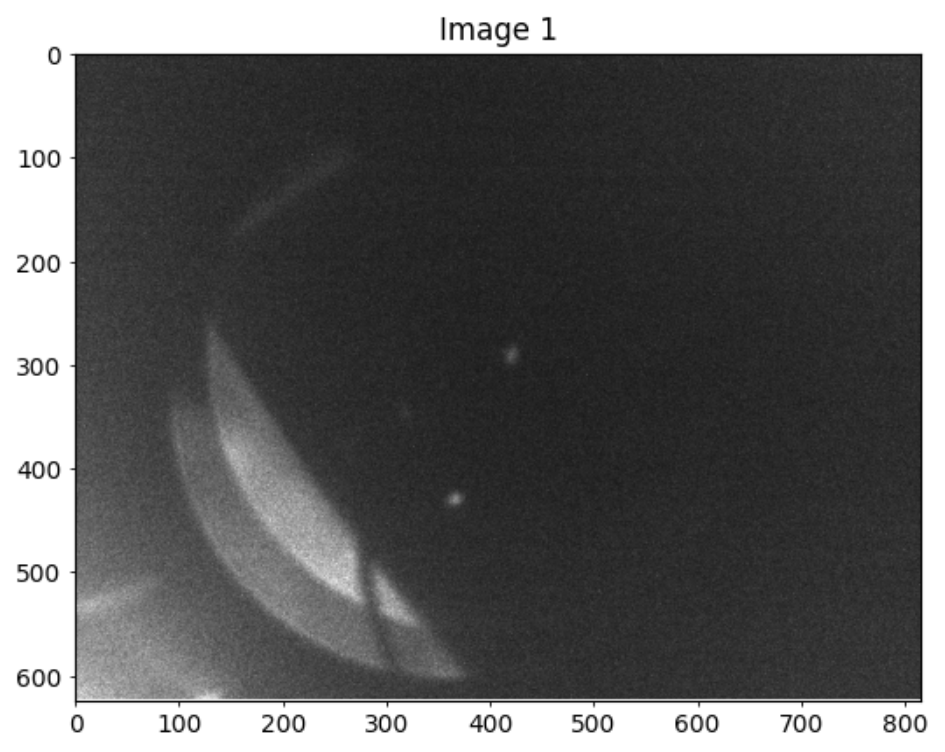
\includegraphics[scale=0.75]{assets/figures/MesuresResultats/ImageSimple.png}
    \caption{Image sent by the camera}
    \label{fig:MES_Ima1}
\end{figure}
An image is recovered using the camera (figure \ref{fig:MES_Ima1}). This image was taken on an "artificial" star, as the weather
was poor during the test phase. The two stars are easy to recognize.
\newpage
Next, a series of 100 images were recovered.
Once all 100 images had been taken, a visual check was carried out to validate the movement of the stars on the screen.
As the background disturbed the basic image (images taken during the day), it was decided to crop it around the
2 stars to remove the bright part (bottom left). The result is shown in Figure \ref{fig:MES_ImaMoy}.
\begin{figure}[H]
    \centering
    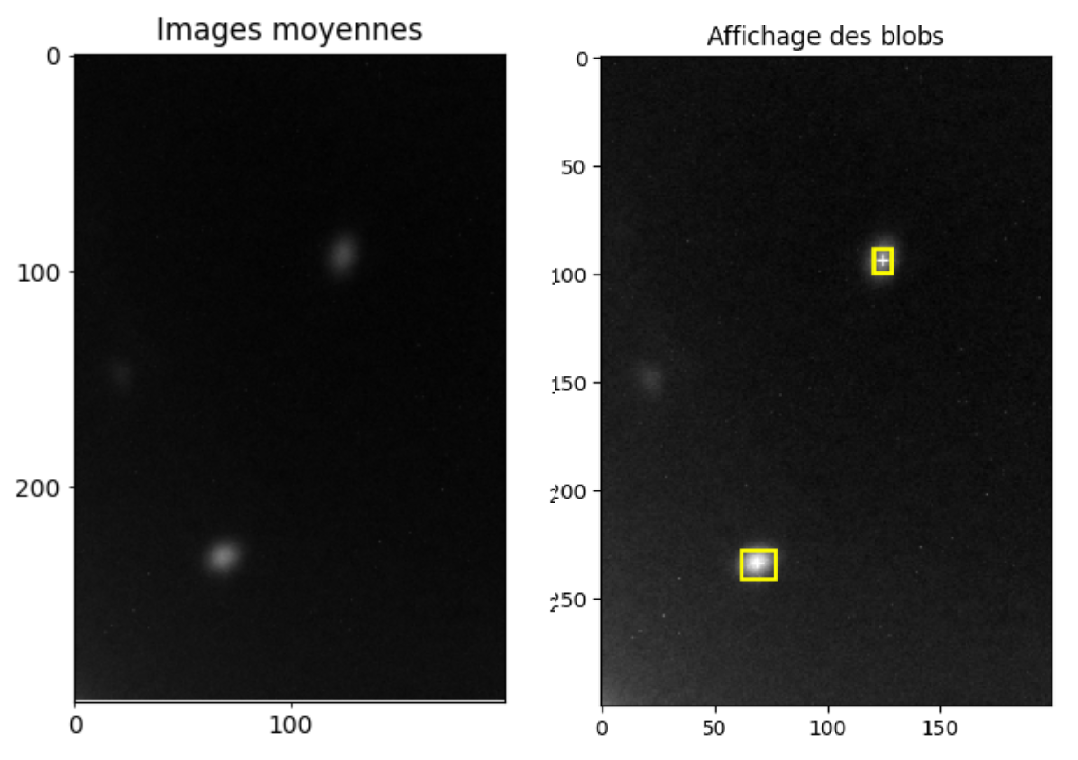
\includegraphics[scale=0.95]{assets/figures/MesuresResultats/ImageMoyenne.png}
    \caption{Addition of all images and star location}
    \label{fig:MES_ImaMoy}
\end{figure}
Figure \ref{fig:MES_ImaMoy} also shows the image used to initialize the system. It contains the 100 images summed and rescaled in values from 0 to 255.
The next step is to locate the 2 stars and find their centroid.
Once initialization is complete, the 2 centroids will be stored in memory, along with the star radii, so that they can
be differentiated.
\newpage
\section{Measurement}
The steps described above (Section \ref{sec:MES_TIS}) will then be carried out for each measurement image.
The stars must be located and their centroids determined (as shown in Figure \ref{fig:MES_ImaMoy}).
\begin{figure}[H]
    \centering
    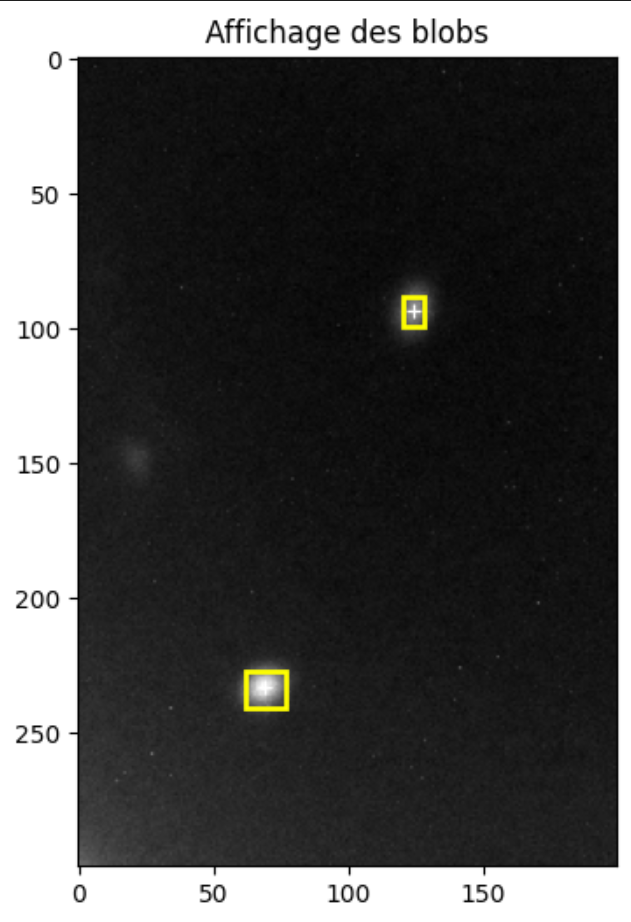
\includegraphics[scale=0.75]{assets/figures/MesuresResultats/BlobsInit.png}
    \caption{Image recognition}
    \label{fig:MES_ImaBlob}
\end{figure}
Each Centroid will be stored in a table specific to the corresponding star.
\newline
Recognition may not work correctly. In this case, the measurement is simply deleted.
However, it would be interesting to add an anomaly detection algorithm later on.
\newpage
\section{Results}
Once all the centroids have been recovered, simply convert them into micrometers to see how the star moves in relation to the turbulence.
\newline
The results of the variations according to the coordinates of the measurements are shown in Figure \ref{fig:MES_VarIm1} and Figure \ref{fig:MES_VarIm2}.
\begin{figure}[H]
    \centering
    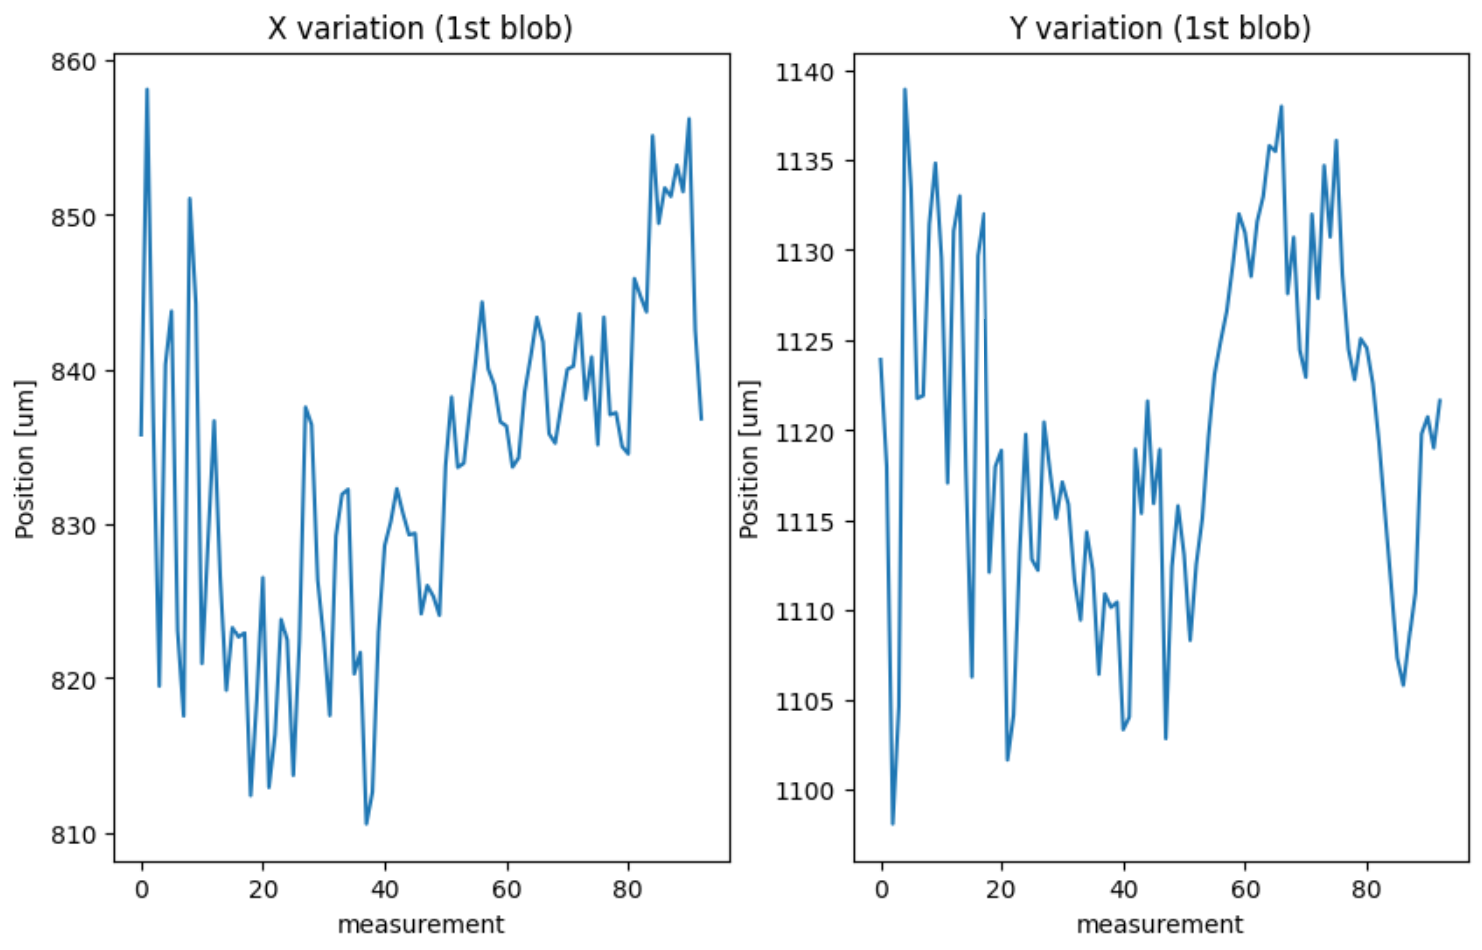
\includegraphics[scale=0.6]{assets/figures/MesuresResultats/VariationImage1.png}
    \caption{Coordinate variation (Image 1)}
    \label{fig:MES_VarIm1}
\end{figure}

\begin{figure}[H]
    \centering
    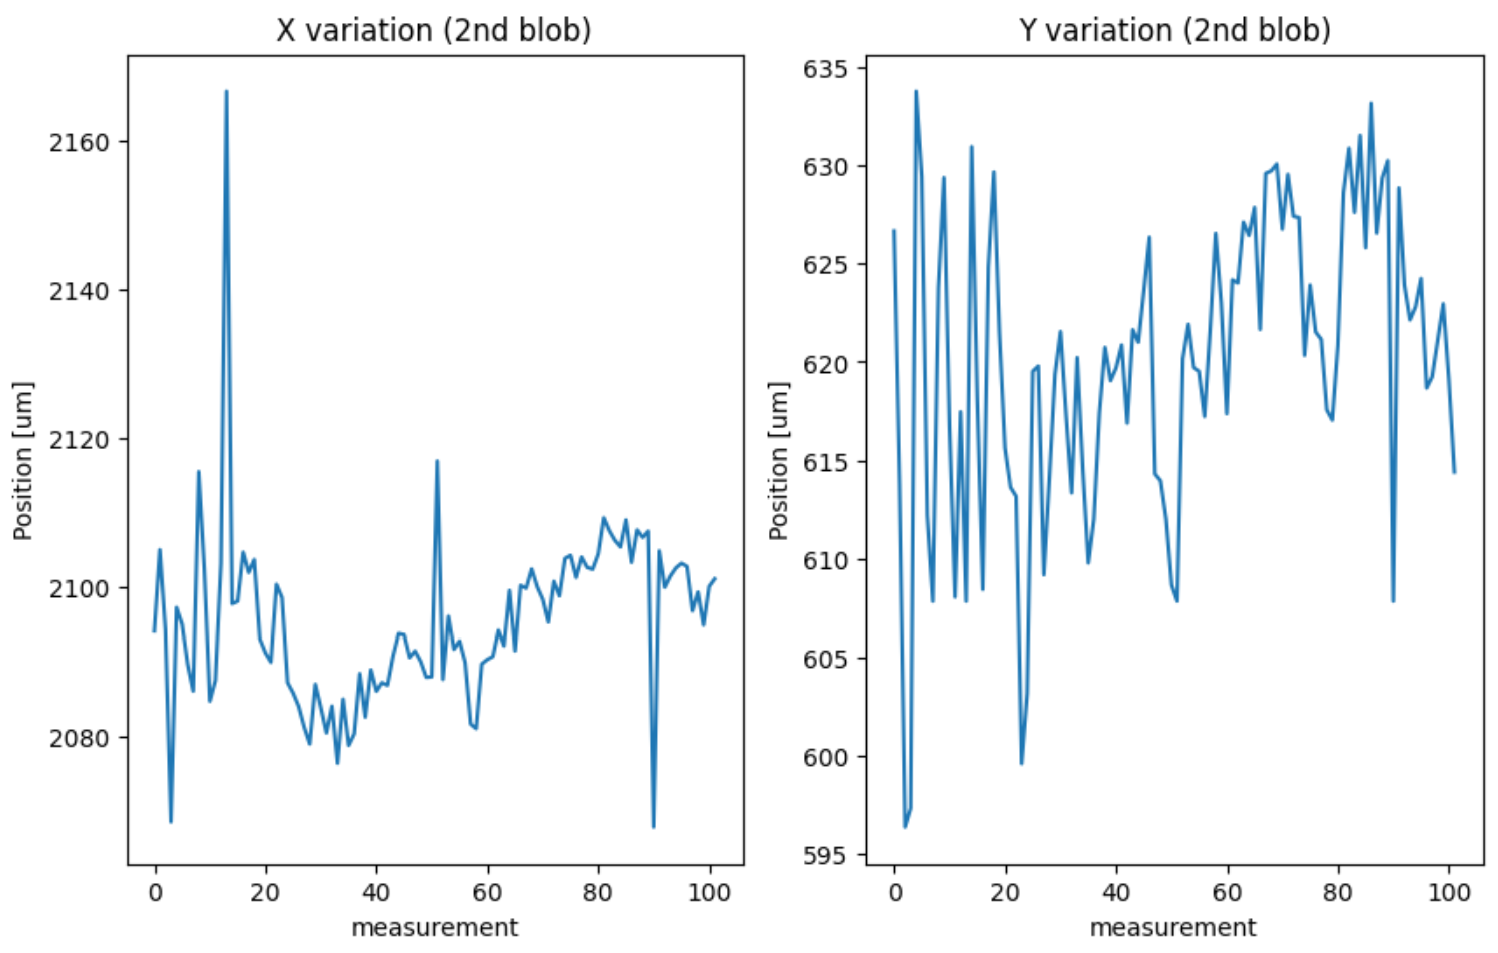
\includegraphics[scale=0.6]{assets/figures/MesuresResultats/VariationImage2.png}
    \caption{Coordinate variation (Image 2)}
    \label{fig:MES_VarIm2}
\end{figure}
\newpage
It's also interesting to represent the centroid of the 2 stars according to their position on the screen. 
In the 2 figures below (\ref{fig:MES_VarCenter1} and \ref{fig:MES_VarCenter2}), the initialization centroids are 
shown in blue and the measurement centroids in red.
\begin{figure}[H]
    \centering
    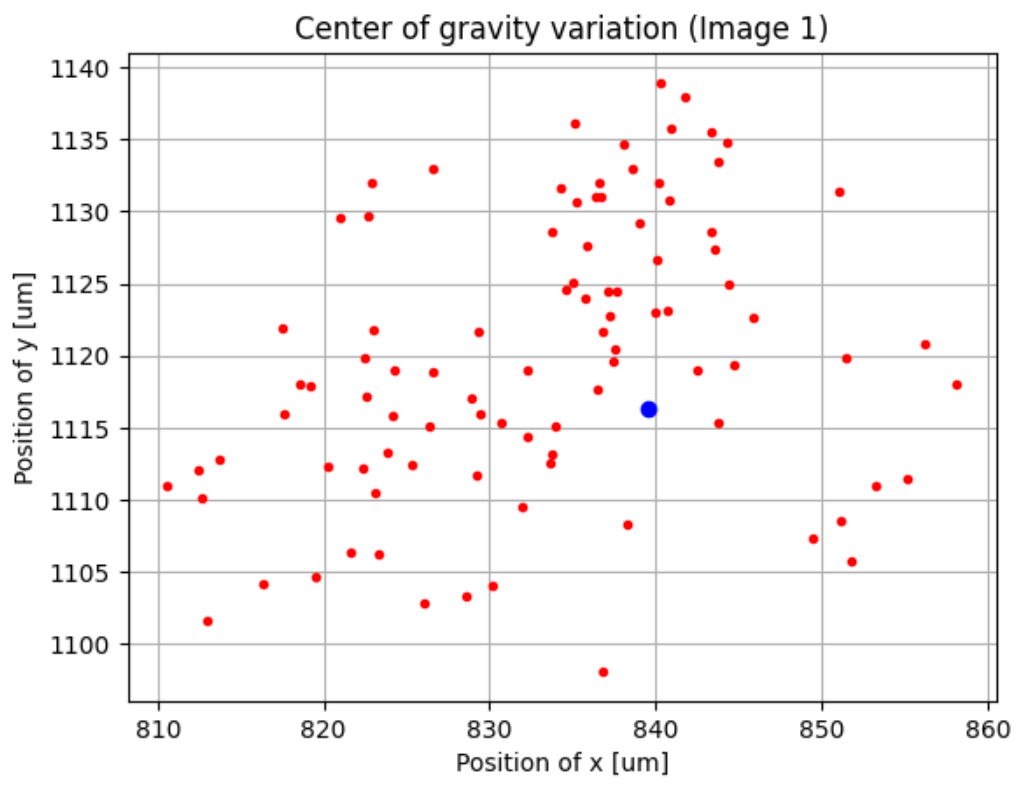
\includegraphics[scale=0.65]{assets/figures/MesuresResultats/VariationCenter1.png}
    \caption{Shifting centers of gravity (Image 1)}
    \label{fig:MES_VarCenter1}
\end{figure}

\begin{figure}[H]
    \centering
    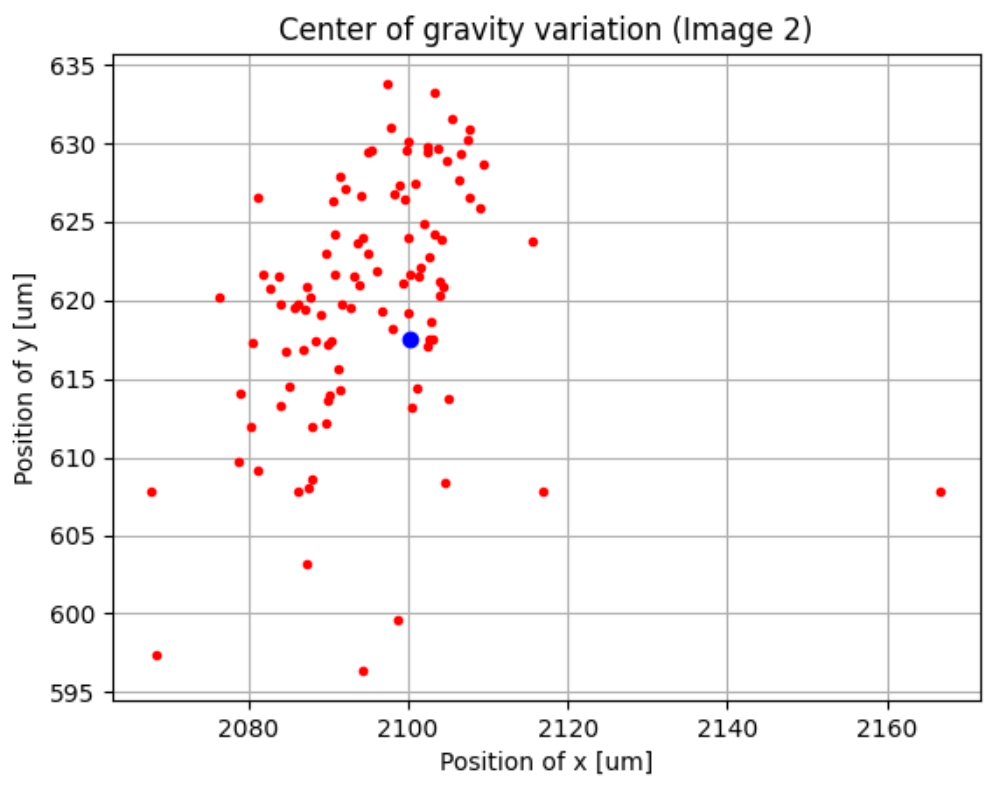
\includegraphics[scale=0.65]{assets/figures/MesuresResultats/VariationCenter2.png}
    \caption{Shifting centers of gravity (Image 2)}
    \label{fig:MES_VarCenter2}
\end{figure}
The measurements of the centroids in the second image have a value that seems out of line. It will therefore not be analyzed 
in the following section (\ref{sec:ANAL_Pos}). 
These errors may occur despite the protection implemented. 
This is due to the image processing and star recognition algorithms.
This algorithm will be modified to make it more reliable in the future. As it stands, however, it still contains a few bugs.